\documentclass[letterpaper, 10 pt, conference]{ieeeconf}

\IEEEoverridecommandlockouts

\overrideIEEEmargins

\makeatletter
\let\NAT@parse\undefined
\makeatother

\usepackage[dvipsnames]{xcolor}

\newcommand*\linkcolours{ForestGreen}

\usepackage{times}
\usepackage{graphicx}
\usepackage{amssymb}
\usepackage{gensymb}
\usepackage{amsmath}
\usepackage{breakurl}
\def\UrlBreaks{\do\/\do-}
\usepackage{url,hyperref}
\hypersetup{
colorlinks,
linkcolor=\linkcolours,
citecolor=\linkcolours,
filecolor=\linkcolours,
urlcolor=\linkcolours}

%\usepackage{algorithm}
\usepackage[]{algorithm2e}
\usepackage{algorithmic}

\usepackage[labelfont={bf},font=small]{caption}
\usepackage[none]{hyphenat}

\usepackage{mathtools, cuted}

\usepackage[noadjust, nobreak]{cite}
\def\citepunct{,\,}

\usepackage{tabularx}
\usepackage{amsmath}

\usepackage{float}

\usepackage{pifont}
\newcommand{\cmark}{\ding{51}}%
\newcommand{\xmark}{\ding{55}}%

\newcommand*\diff{\mathop{}\!\mathrm{d}}
\newcommand*\Diff[1]{\mathop{}\!\mathrm{d^#1}}
\newcommand*\imgres{600}

\newcommand*\GitHubLoc{https://github.com/Jeffrey-Ede/ALRC}

\newcolumntype{Y}{>{\centering\arraybackslash}X}


\usepackage[]{placeins}

\newcommand\extraspace{3pt}

\usepackage{placeins}

\usepackage{tikz}
\newcommand*\circled[1]{\tikz[baseline=(char.base)]{
            \node[shape=circle,draw,inner sep=0.8pt] (char) {#1};}}
            
\usepackage[framemethod=tikz]{mdframed}

\usepackage{afterpage}

\usepackage{stfloats}

\usepackage{atbegshi}
\newcommand{\handlethispage}{}
\newcommand{\discardpagesfromhere}{\let\handlethispage\AtBeginShipoutDiscard}
\newcommand{\keeppagesfromhere}{\let\handlethispage\relax}
\AtBeginShipout{\handlethispage}

\usepackage{comment}

\title{\LARGE \bf
\textit{Fog@Home}: Toward a Volunteer Fog Computing infrastructure \\running on commodity hardware
}

\author{Contributors$^{1}$% <-this % stops a space
\\IMT Atlantique, France
\\jonathan.pastor@imt-atlantique.fr
}


\begin{document}


\maketitle
\thispagestyle{empty}
\pagestyle{empty}


%%%%%%%%%%%%%%%%%%%%%%%%%%%%%%%%%%%%%%%%%%%%%%%%%%%%%%%%%%%%%%%%%%%%%%%%%%%%%%%%
\begin{abstract}
With the advent of \textit{Cloud Computing}, IT applications have adopted complex architectures composed of many software services leveraging in computing infrastructures hosted in large datacenters. 
To meet economies of scale and reduce operational costs, these large datacenters are located in places where energy price is affordable.
These locations are often located far from population centers, leading to an important network latency between hosted services and end users.
\textit{Fog Computing} is a paradigm that proposes to extend \textit{Cloud Computing}'s large datacenters with smaller datacenters located close to population centers : latency-critical applications are intended to be hosted in these smaller datacenters, while non latency-critical applications will be hosted in classical datacenters.
In this article we propose a framework that enables to build distributed \textit{Fog Computing} infrastructure, with a functioning inspired by \textit{Volunteer Computing}, which has low hardware requirements.
\end{abstract}

%%%%%%%%%%%%%%%%%%%%%%%%%%%%%%%%%%%%%%%%%%%%%%%%%%%%%%%%%%%%%%%%%%%%%%%%%%%%%%%%
\section{Introduction}
In this article we propose \textit{Fog@Home}, a framework that can set up an infrastructure at the intersection between \textit{Fog computing} infrastructures and \textit{Volunteer Computing} infrastructures.
Les infrastructures de type Fog Computing sont de plus en plus utilisées, par exemple, dans les villes intelligentes. Ces infrastructures sont complexes au sens où elles mettent en oeuvre une grande diversité d'éléments (différents capteurs, unités de calcul de faible consommation) en grand nombre (par ex, gestion des feux de signalisation d'une grande métropole). Dans l'objectif de tester le déploiement d'un outil opérant dans le Fog Computing ou à des fins de recherches pour l'étude de ces infrastructures, nous avons besoin d'infrastructures géo-distribuées et possédant un nombre important d'éléments facilement accessibles.

Pour un seul acteur, une telle plate-forme peut s'avérer difficile à mettre en place (installation d'éléments à l'échelle nationale) et coûteuse (nombre conséquent d'appareils à acquérir - switch, capteurs de différents types, unité de calcul et de stockage). Cependant, pour une communauté composée de plusieurs acteurs, une telle infrastructure peut-être vue comme un agrégat de petites entités que nous appellerons, fog cluster. Il est alors envisageable que chaque acteur ajoute un fog cluster à l'infrastructure pour un investissement financier faible. En effet, pour contribuer à une architecture IaaS de type Grid5000, les acteurs doivent acheter du matériel coûteux (serveur, climatisation) et les coûts de maintenance sont eux aussi élevés (consommation électrique, administrateur, remplacement de matériel). Pour une infrastructure de fog, cette contribution est moindre car le matériel est peu coûteux (capteurs, nano-ordinateurs - single-board computer) et les coûts de maintenance associés sont faibles (consommation énergétique basse, pièces de rechange peu onéreuses). Pour ces raisons, une communauté d'une centaine d'acteurs à l'échelle d'un pays se rassemblant pour créer une infrastructure commune nous semble réaliste et prometteuse. Chaque acteur pourrait alors contribuer à l'infrastructure en hébergeant un fog cluster dans sa structure (université, entreprise) et, ainsi, profiter des ressources de toute la communauté. 

Dans cet article, nous présentons la première brique de cette infrastructure collaborative de fog computing : le fog cluster. Nous allons détailler le matériel nécessaire à la création de ce cluster ainsi que la solution logicielle développée pour sa gestion. Enfin, nous évaluerons les performances du gestionnaire de ressources du cluster en comparant différente configuration possible. Nous finirons par évoquer les futures étapes et réflexions nécessaires à la création de cette plate-forme de fog computing collaborative.

%%%%%%%%%%%%%%%%%%%%%%%%%%%%%%%%%%%%%%%%%%%%%%%%%%%%%%%%%%%%%%%%%%%%%%%%%%%%%%%%
\section{Architecture Matérielle}
\label{sec:architecture}
La plate-forme de fog computing présentée dans cet article peut être vue comme l'agrégation de fog clusters connectés entre eux via Internet, c'est-à-dire, une liaison de qualité variable. Chaque fog cluster va apporter ses ressources à l'infrastructure et, en contrepartie, pouvoir consommer les ressources offertes par les autres clusters.
Le matériel proposé pour la configuration d'un cluster est rapide à installer et facile à administrer tout en offrant la flexibilité nécessaire pour s'adapter à de nombreux cas d'utilisation. Son prix, peu élevé, permet à de nombreux acteurs de rejoindre rapidement la plate-forme et aussi de diminuer son coût de fonctionnement facilitant ainsi le remplacement des pièces défaillantes. Pour atteindre ces objectifs, nous avons choisi de baser la plate-forme sur les populaires Raspberry Pi connectés à l'aide d'un switch PoE (Power over Ethernet).

L'avantage majeur des Raspberry Pi est la possibilité de les alimenter en PoE à partir de la carte réseau. Grâce à la technologie PoE, le switch est capable d'alimenter les  Raspberry ce qui diminue le nombre de câbles et de prises nécessaires à l'alimentation du cluster. Les Raspberry sont donc connectés au switch avec un câble Ethernet qui fournit l'alimentation et la connexion au réseau. De plus, la possibilité de contrôler l'alimentation des ports PoE du switch via le protocole SNMP permet d'éteindre et d'allumer les Raspberry très facilement. Les Raspberry Pi ont aussi été choisis car nous étions à la recherche d'un nano-ordinateur supportant le boot PXE afin de choisir le système d'exploitation à exécuter au démarrage. Le PoE et le boot PXE nous offrent alors de vastes possibilités de configuration des Raspberry.

Nous avons testé des Raspberry Pi 3B+ (2GB de RAM) et les Raspberry Pi 4 (4Gb de RAM). Lors du choix des Raspberry, il faut s'assurer que le modèle choisi prend bien en charge la technologie PXE. Pour la prise en charge du PoE, il faut ajouter des cartes PoE HAT qui se montent sur les Raspberry. Nous avons aussi ajouté une carte micro-SD de 32 Gb ce qui nous laisse 30 Gb de libre après installation d'un système d'exploitation Raspbian.

Le switch choisi doit supporter la technologie PoE sur un maximum de port. Il faut bien vérifier que le power budget du switch est suffisant pour alimenter tous les Raspberry connectés. D'après les tests de consommation réalisés~\ref{ici}, un Raspberry Pi consomme au maximum 8~W. Un switch disposant de 8 ports PoE doit donc avoir un power budget d'au minimum 64~W (8 x 8~W).

Avec cette configuration, il est possible d'acheter le matériel nécessaire pour créer un fog cluster de 8 Raspberry Pi 4 (4Gb de RAM) pour un peu moins de 1000 euros~\ref{facture_annexe}. De plus en plus de systèmes d'exploitation et de logiciels supportent les processeurs ARM, un large choix d'utilisation du cluster est alors possible: bases de données, blockchain, virtualisation, etc. Afin de diminer les coûts d'administration de la plate-forme, nous proposons dans la suite de cette article, une solution logicielle OpenSource de gestion des ressources du clusters. Nous sommes convaincus qu'une pile logicielle commune à tous les clusters diminuera le temps d'administration de chaque cluster en favorisant l'entraide entre les participants et la stabilité du code.

%%%%%%%%%%%%%%%%%%%%%%%%%%%%%%%%%%%%%%%%%%%%%%%%%%%%%%%%%%%%%%%%%%%%%%%%%%%%%%%%
\section{Noeud de service}
\label{sec:gestionnaire}
Le fog cluster construit avec le matériel listé ci-dessus dispose donc de 8~noeuds Raspberry~Pi~4. Sur ces 8~noeuds, un des noeuds sera utilisé comme noeud de service et les 7~autres noeuds seront les noeuds ressources que les utilisateurs pourront réserver.

Le noeud de service établit le lien entre les utilisateurs et les noeuds ressources. Le noeud de service utilise des outils très répandus comme \textit{dnsmasq}, \textit{mariaDB}, \textit{NFS}. Ces outils permettent de configurer les services suivants :
\begin{itemize}
    \item un serveur DHCP définissant les adresses IP des noeuds ressources ;
    \item un serveur PXE hébergeant les différents systèmes d'exploitation à installer sur les noeuds ressources ;
    \item un serveur NFS utiliser pour démarrer les noeuds tout en pouvant formater leur stockage interne ;
    \item le gestionnaire de ressources du cluster qui permet aux utilisateurs de réserver des ressources ;
    \item une base de données pour enregistrer les comptes utilisateurs et gérer la configuration des noeuds ressources ;
\end{itemize}

Pour configurer les noeuds ressources, le gestionnaire doit avoir connaissance de l'architecture du fog cluster. Plusieurs informations sont décrites à l'aide de fichiers JSON pour assurer le bon fonctionnement du gestionnaire. Pour les switchs~\ref{switch_json} des noeuds ressources, les informations nécessaires aux connexions SNMP sont renseignées. Le gestionnaire peut alors activer et désactiver l'alimentation PoE des ports ce qui permet d'éteindre et d'allumer les noeuds. La description des noeuds ressources~\ref{noeud_json} précise le port du switch sur lequel le noeud est branché ainsi que son identifiant utilisé lors du boot PXE. Des informations sur chaque système d'exploitation à installer~\ref{env_json} sont nécessaires afin de configurer correctement les partitions après avoir copié le système sur le noeud ressource.
Pour pouvoir faciliter l'ajout de nouvelles ressources, chaque élément (switch, ressource, environnement) est décrit dans un fichier JSON indépendant. Après l'installation du gestionnaire de ressources, l'administrateur de l'infrastructure doit fournir une description des ressources disponibles. Pour cela, il peut soit remplir les fichiers de description manuellement, soit utiliser la page d'administration du gestionnaire. À partir de cette page d'administration, l'administrateur va pouvoir ajouter des switchs en renseignant leur adresse IP et les informations nécessaires à l'utilisation du protocole SNMP (communauté, OID des ports PoE). Pour chaque switch, l'administrateur pourra alors éteindre et allumer les ports PoE et lancer la détection de ressources sur un ou plusieurs ports. Ces outils d'administration permettent de remplir les fichiers JSON décrivant les switchs et les noeuds ressources. Les fichiers décrivant les environnements, évoluant plus rarement, sont à remplir manuellement.

Une fois configuré, le gestionnaire de ressources sert de point d'entrée aux utilisateurs de la plate-forme de fog computing. Cet outil va permettre aux utilisateurs de s'authentifier afin d'avoir accès aux ressources de la plate-forme. Un utilisateur authentifié peut sélectionner des ressources disponibles puis choisir un environnement, c'est-à-dire, un système d'exploitation et une configuration logicielle, à déployer. Une fois l'environnement déployé, l'utilisateur à un accès administrateur à son noeud.

Pour déployer un environnement, le gestionnaire a besoin de deux fichiers : le fichier image du système d'exploitation incluant une configuration logicielle spécifique ainsi que le fichier~JSON décrivant l'environnement. À partir de ces fichiers, le gestionnaire va ensuite exécuter une liste de commandes en se connectant avec le protocole SSH sur chaque noeud ressource à configurer. Pour exécuter ces commandes, le gestionnaire de ressources fait passer le noeud par une séquence d'états prédéfinis~\ref{fig:states}. Chaque état~\ref{etat_json} est composé d'un nom, d'une série de commandes à exécuter et d'une condition à vérifier pour que le noeud passe à l'état suivant. Tant que la condition n'est pas vérifiée, l'état du noeud n'est pas modifié. Chaque état possède un timeout qui est utilisé pour détecter les blocages lors du déploiement. Lorsque ce timeout expire, le noeud est soit redémarré pour essayer de continuer le déploiement, soit considéré comme perdu. Dans ce cas, l'utilisateur peut choisir de redéployer son environnement ou de libérer le noeud. L'utilisation de ces états permet aux utilisateurs de suivre le déploiement des ressources demandées. Les états simplifient aussi la détection et la correction de pannes lors des déploiements. Dans l'exemple illustré par la figure~\ref{diagramme_etats}, on voit les états parcourus par les noeuds lors de la configuration de l'environnement Raspbian Buster. En cas d'expiration du timeout dans l'état \textit{user\_conf}, le gestionnaire de ressources va redémarrer le noeud en coupant puis rétablissant l'alimentation du port PoE. La condition de l'état \textit{user\_conf} sera alors à nouveau tester. Si le timeout expire une seconde fois, le noeud passera dans l'état \textit{lost}.

\begin{figure}[htb]
  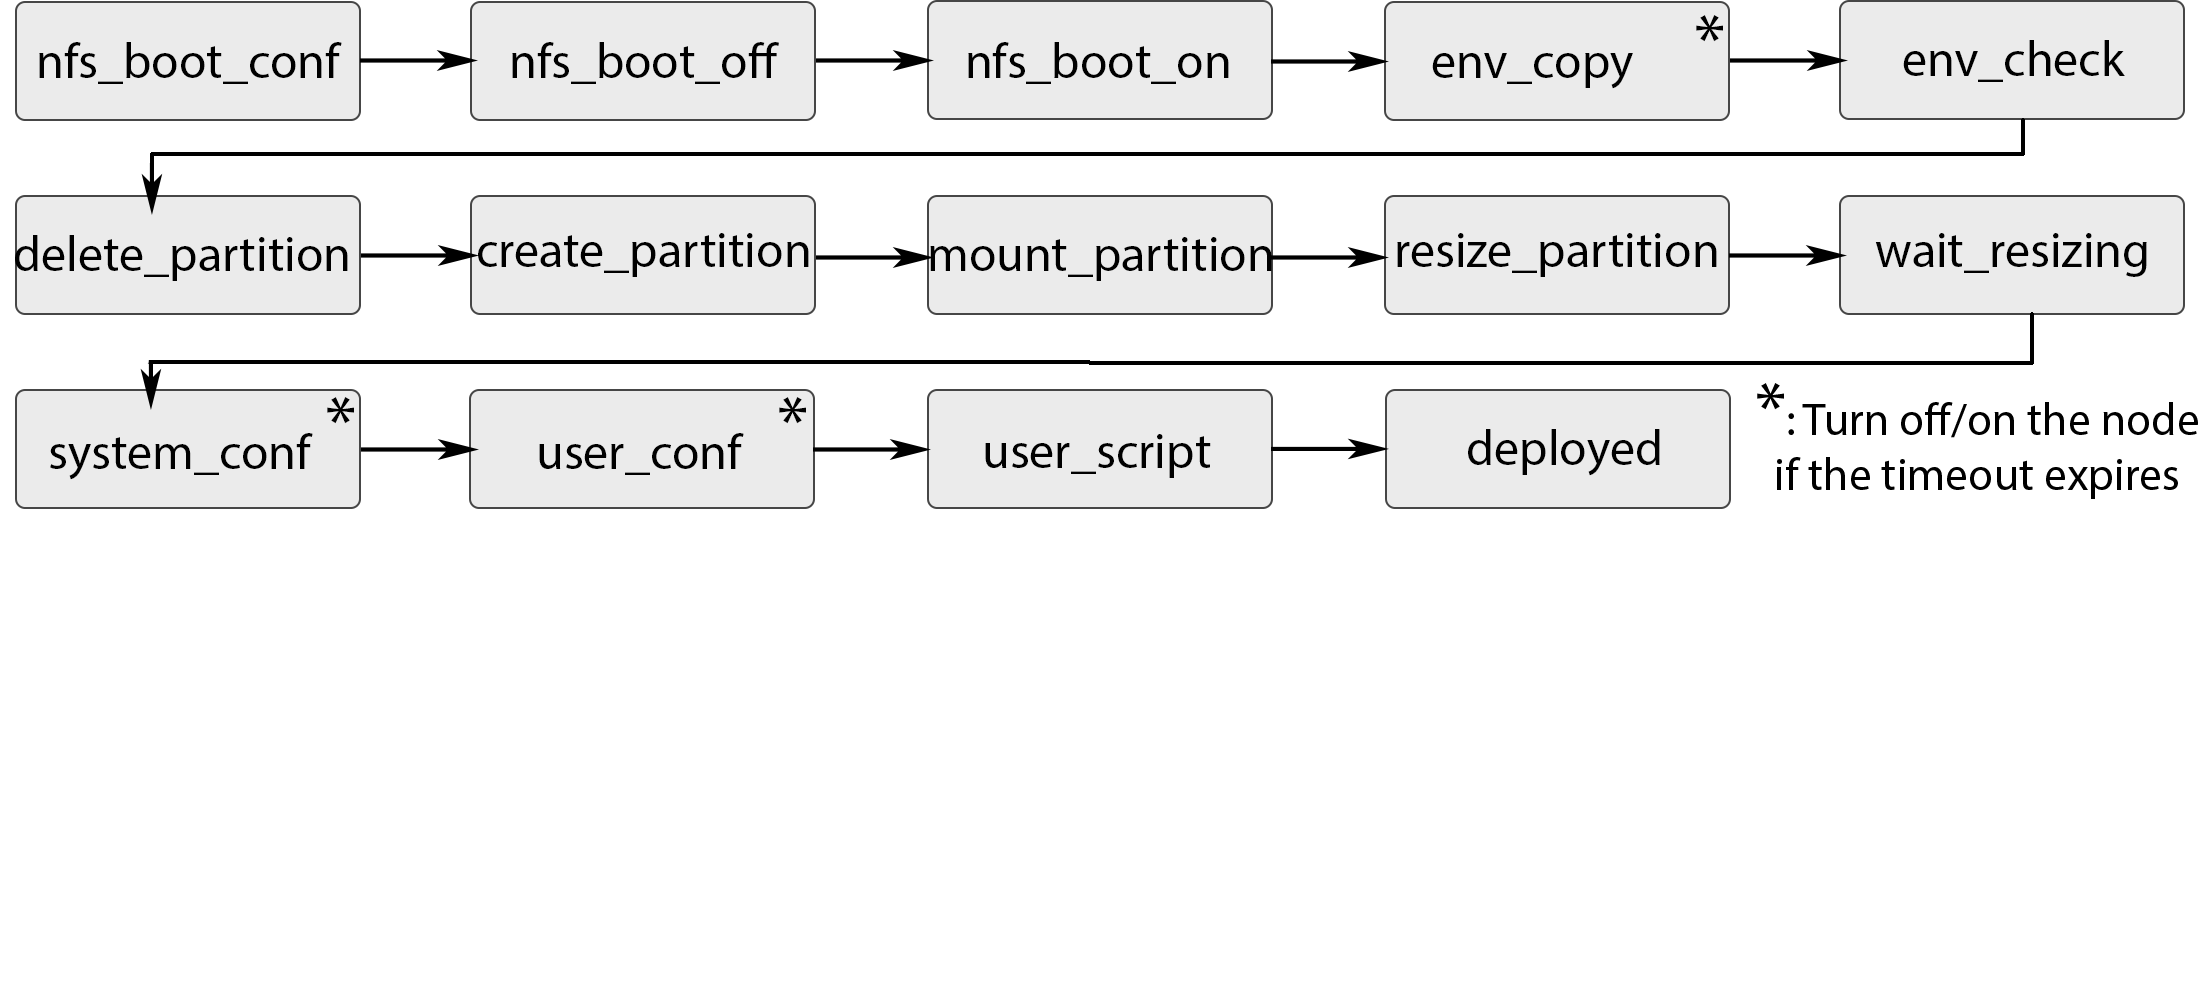
\includegraphics[width=\linewidth, height=100pt]{img/states.png}
  \caption{States used to follow the deployment process}
  \label{fig:states}
\end{figure}

Afin de faciliter l'installation du fog cluster, nous avons créé une image d'un système Raspbian 32-bits incluant le gestionnaire de ressources. Cette image peut-être téléchargée et copiée sur un Raspberry Pi du cluster afin de déployer rapidement le gestionnaire de ressources. La configuration des noeuds ressources et la gestion des utilisateurs se feront alors à l'aide du compte administrateur existant. Le gestionnaire de ressources peut facilement être mis à jour en récupérant la dernière version à partir de notre dépôt GitHub (\url{https://github.com/remyimt/seduce\_pp}).

%%%%%%%%%%%%%%%%%%%%%%%%%%%%%%%%%%%%%%%%%%%%%%%%%%%%%%%%%%%%%%%%%%%%%%%%%%%%%%%%
\section{Automatisation des déploiements des environnements}
\label{sec:os_install}

Le gestionnaire de ressources sert à installer différents systèmes d'exploitation sur les noeuds ressources du cluster. Ces systèmes d'exploitation sont distribués sous forme d'images à copier sur le stockage interne du Raspberry, c'est-à-dire, le plus souvent, une carte SD ou un disque USB. Les images fournies par les distributeurs (Raspbian, Ubuntu, etc.) peuvent être utilisées sans modification sur le cluster. Cependant, afin d'améliorer les temps de déploiement, nous compressons ces images avec l'outil bzip. Afin de pouvoir copier l'image du système d'exploitation sur le stockage interne du Raspberry, le Raspberry doit être démarré à partir d'un disque externe. Dans notre cas, nous avons choisi de démarrer une première fois le Raspberry à partir d'un serveur NFS afin de copier le nouveau système. Après la copie, le Raspberry est redémarré à partir de son stockage interne.

Dans cette section, nous allons détailler le processus de démarrage d'un noeud Raspberry du cluster. Nous nous intéresserons en particulier aux mécanismes permettant de choisir un démarrage sur le serveur NFS ou sur le stockage interne du Raspberry.

Au début de la phase de démarrage d'un nano-ordinateur de marque Raspberry, plusieurs fichiers sont chargés afin de configurer le bootloader. Lors d'un démarrage à partir d'une carte SD, ces fichiers sont copiés sur  copie du système d'exploitation, par exemple,  présents dans la première partition de la carte après avoir copié un système d'exploitation.


Pour pouvoir choisir l'environnement chargé au démarrage des noeuds, les noeuds sont configurés pour récupérer leur environnement de démarrage sur un serveur PXE distant. Cet environnement comprend plusieurs fichiers de configuration, notamment le fichier \textit{cmdline.txt} que nous utilisons pour démarrer un noeud soit sur le serveur NFS, soit sur son stockage interne. Ces fichiers de configuration sont présents dans les images des systèmes d'exploitation. Par exemple, dans les images raspiOS (anciennement, Raspbian), les fichiers de configuration sont situés dans la première partition de l'image. Ces fichiers sont donc copiés sur notre serveur PXE et les noeuds sont configurés pour toujours demander ces fichiers lors de leur démarrage. Pour l'installation du système d'exploitation du noeud, nous démarrons donc le noeud à partir du serveur NFS et nous pouvons alors nous connecter sur le noeud afin de copier l'image du système d'exploitation de notre choix sur le stockage interne.
Afin de gérer le démarrage de plusieurs noeuds simultanément, nous créons un dossier de démarrage par noeud. Le nom de ce dossier doit être l'identifiant du noeud obtenu en lisant la propriété \textit{Serial} du fichier \textit{/proc/cpuinfo}.

Une fois la copie du nouveau système d'exploitation effectuée, la partition système du noeud est montée sur le système NFS afin de pouvoir configurer le noeud pour son utilisation future. Par exemple, nous ajoutons les clés SSH du gestionnaire et de l'utilisateur pour avoir un accès administrateur sur le nouveau système.

Après cette phase de configuration, nous réalisons l'extension de la partition système existante afin qu'elle utilise la totalité de l'espace de stockage disponible. Cette opération est traditionnellement faite au premier démarrage du noeud après l'installation du système. Cependant, n'ayant pas de connexion à l'interface graphique, nous préférons effectuer cette opération à partir du système monté en NFS.

Après ces opérations, le noeud est redémarré puis mis à la disposition de l'utilisateur.

%%%%%%%%%%%%%%%%%%%%%%%%%%%%%%%%%%%%%%%%%%%%%%%%%%%%%%%%%%%%%%%%%%%%%%%%%%%%%%%%
\section{Évaluation}
\label{sec:implementation}

\subsection{Description de l'environnement de test}
Le gestionnaire de ressources est une application codée en Python3 utilisant le module Flask pour la génération de l'interface web. Il est composé de deux services : \textit{pitasks} et \textit{pifrontend}. Le service \textit{pifrontend} fournit l'interface web utilisé par les utilisateurs et les administrateurs pour utiliser la plate-forme. Le service \textit{pitasks} est responsable de déployer les environnements sur les noeuds ressources. Le code de ces deux services est disponible sur notre dépôt Github à l'adresse suivante \textit{http://github.com/remyimt/seduce\_pp}. Pour cette évaluation, nous utiliserons vingt noeuds ressources de type Raspberry Pi 3B~plus avec 2~Go de mémoire. Sur ces noeuds, nous allons déployer l'image Raspbian qui est un système d'exploitation basé sur Debian optimisé pour fonctionner sur les différents Raspberry Pi. Nous avons choisi la version Lite de Raspbian qui ne comporte pas d'interface graphique. Deux modifications ont été apportées à l'image Raspbian: la suppression du fichier \textit{bootcode.bin} et l'activation par défaut du serveur SSH.

Le fichier \textit{bootcode.bin} se trouve dans la première partition de l'image Raspbian. Si ce fichier est copié sur la carte SD des Raspberry, ils n'effectueront plus la phase de boot PXE qui est nécessaire pour tous les noeuds ressources. Nous préférons donc supprimer ce fichier de l'image.

Après l'installation du système Raspbian sur les noeuds, les utilisateurs se connectent à leurs noeuds à l'aide de connexions SSH. Il est donc impératif que ce service soit lancé au démarrage de tous les systèmes installés sur les noeuds. Sur Raspbian, l'activation de ce service au démarrage est fait par l'ajout d'un fichier nommé \textit{ssh} dans la partition \textit{boot} (la première partition de l'image). Une fois ces  modifications effectuées, l'image Raspbian est ajoutée au gestionnaire de ressource en créant le fichier JSON décrivant l'environnement.

Afin de tester le gestionnaire de ressources et l'infrastructure du fog cluster, nous allons déployer l'environnement Raspbian sur plusieurs noeuds en parallèle. À la fin des déploiements, nous vérifions la configuration correcte de chaque noeud en effectuant une connexion SSH sur ce noeud. Si la connexion sur le noeud est possible, nous considérons que le déploiement est réussi.

Pour chaque déploiement effectué, nous notons la réussite ou l'échec du déploiement et, en cas de succès, le temps en secondes du déploiement. Notre expérience visant à mesurer l'impact de la parallélisation des déploiements se déroule en 5~étapes :
\begin{itemize}
    \item le déploiement en parallèle de l'environnement RaspiOS~32-bit sur 4 Raspberry Pi 3 B+ ;
    \item le déploiement en parallèle de l'environnement RaspiOS~32-bit sur 8 Raspberry Pi 3 B+ ;
    \item le déploiement en parallèle de l'environnement RaspiOS~32-bit sur 12 Raspberry Pi 3 B+ ;
    \item le déploiement en parallèle de l'environnement RaspiOS~32-bit sur 16 Raspberry Pi 3 B+ ;
    \item le déploiement en parallèle de l'environnement RaspiOS~32-bit sur 20 Raspberry Pi 3 B+ ;
\end{itemize}
Comme tous les noeuds partagent le même lien réseau et la même stockage NFS pendant leur configuration, plus le nombre de noeuds déployés en parallèle augmente, plus les temps de déploiements sont longs.

De plus, les quantités de ressources CPU et mémoire disponibles pour exécuter le gestionnaire de ressources influencent aussi les temps de déploiement. Pour mesurer cet impact, nous avons exécuté notre expérience en exécutant le gestionnaire de ressources sur 3~architectures différentes : une machine virtuelle KVM disposant de 4~vCPU et 4~Go de mémoire ; un Raspberry~Pi~3B+ disposant de 2~Go de mémoire et un Raspberry~Pi~4 disposant de 4~Go de mémoire. Nous avons exécuté plusieurs fois notre expérience. Les moyennes des temps de déploiements obtenus sont présentés dans le tableau~\ref{fig:dtime}.

\begin{figure}[htb]
  \includegraphics[width=\linewidth]{img/deployment-times.pdf}
  \caption{Temps de déploiement sur 3 architectures distinctes}
  \label{fig:dtime}
\end{figure}

D'après ces résultats, nous observons que les déploiements opérés depuis la VM sont plus rapides que ceux effectués à partir des Raspberry. De plus, lorsqu'on déploie 20 noeuds simultanément à partir des Raspberry, certains déploiements échouent. Lors de l'échec d'un déploiement, l'utilisateur ne peut pas accéder à sa ressource qui doit donc être redéployée.

Contrairement à nos attentes, les déploiements effectués à partir du Raspberry Pi 4 ne sont pas plus rapides que ceux effectués à partir du Raspberry Pi 3 (possédant deux fois moins de mémoire). On observe même un taux d'échec plus important sur le Raspberry Pi 4. Afin d'identifier le problème, nous avons observé les temps d'exécution de chaque état du déploiement. Afin de simplifier la lecture, les états ont été regroupés en 5~étapes :
\begin{itemize}
    \item Démarrage du noeud sur le stockage NFS hébergé par le gestionnaire de ressources. Cette phase comprend la création du dossier de démarrage du noeud sur le gestionnaire de ressources, l'extinction puis l'activation du port PoE utilisé par le noeud ;
    \item Copie de l'environnement sur la carte SD du Raspberry. Cette phase comprend la copie et la décompression de l'image du système d'exploitation sur la carte SD du noeud ;
    \item Création de la seconde partition. Durant cette phase, la seconde partition du système d'exploitation est supprimée et est recréée avec une taille prenant en compte la taille de la carte SD. La manipulation des partitions est faite avec \textit{fdisk}.
    \item Extension de la seconde partition. Durant cette phase, la table de partition est réécrite afin de prendre en charge la nouvelle taille de la partition. La commande \textit{resize2fs} est exécutée ;
    \item Configuration du système d'exploitation. Cette phase comprend la modification des mots de passe par défaut, la copie des clés SSH de l'utilisateur et la copie des fichiers de démarrage du noeud sur le gestionnaire de ressources (fichiers utilisés pour le démarrage en PXE).
\end{itemize}

Les temps obtenus sont présentés dans le tableau~\ref{fig:stime}. Pour faciliter la comparaison, les temps t indiqués dans le tableau sont relatifs au temps de déploiement de la VM $T_{VM}$ ($t = T_{VM} - T_{Raspberry}$).

\begin{figure}[htb]
  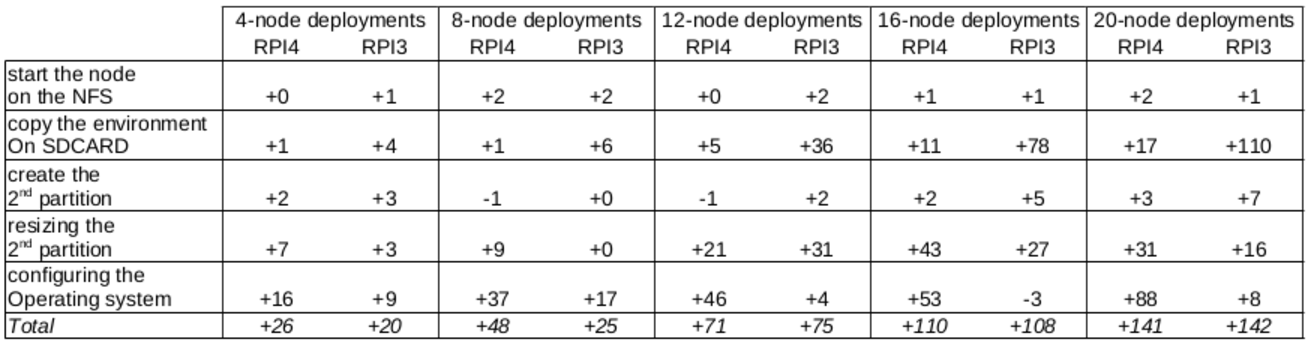
\includegraphics[width=\linewidth]{img/state-times.pdf}
  \caption{Temps passés dans les différents états lors du déploiement}
  \label{fig:stime}
\end{figure}

Lorsque le nombre de noeuds déployés simultanément augmente, on observe une hausse 6 fois plus importante des temps de copie de l'environnent sur le Raspberry Pi 3 que sur le Raspberry Pi 4. Cette hausse est probablement due à la plus faible capacité mémoire du Raspberry Pi 3.

Cependant, les phases d'extensions de la partition et de configuration du système d'exploitation sont respectivement 2 fois et 11 fois plus lente sur le Raspberry Pi 4 que sur le Raspberry Pi 3. Nous n'avons pas d'explications pour expliquer ce phénomène.

Intéressons-nous maintenant aux déploiements ayant échoué lors des déploiements en parallèle de 20~noeuds. Nous considérons qu'un déploiement échoue lorsqu'il reste plus de 180 secondes dans un état autre que l'état de copie de l'environnement.

Lorsque le gestionnaire de ressources est hébergé sur un Raspberry Pi 3, la totalité des noeuds en échec n'ont pas réussi à démarrer sur le système NFS. Le gestionnaire n'arrive donc pas à se connecter en SSH sur les noeuds.

Avec le gestionnaire de ressources hébergé sur un Raspberry Pi 4, 97~\% des noeuds en échec sont dans un des trois états de l'étape de configuration du système d'exploitation. Une hypothèse serait que le système est considérablement ralenti lors de cette étape ce qui empêche la réalisation des tâches en moins de 180 secondes. En augmentant notre limite de temps, on réduirait probablement le nombre de noeuds en échec tout en augmentant davantage le temps passé dans les états de configuration du système.

%%%%%%%%%%%%%%%%%%%%%%%%%%%%%%%%%%%%%%%%%%%%%%%%%%%%%%%%%%%%%%%%%%%%%%%%%%%%%%%%
\section{Conclusion}
1. Comment les fog clusters sont-ils reliés entre eux ? Point centralisé, décentralisé, BDD distribuée
2. Protocole de consommation des ressources : Comment gérer le ratio ressources apportées / ressources consommées ? Calcul des ressources consommées par cluster ou par utilisateur ?
deux niveaux de consommation : une politique de consommation au niveau du cluster (les consommations au niveau de la plate-forme) et une politique de consommation au niveau de l'utilisateur interne au cluster.
3. Quel mécanisme d'authentification ? est-ce qu'un utilisateur peut s'authentifier sur n'importe quel cluster...
4. Mécanisme de réservations : une réservation de moins d'1h peut-être faite instantanément quelque-soit la taille de la réservation. Une réservation consommant moins de 10\% de l'infrastructure
est traitée immédiatement ; une réservation consommant entre 11\% et 30\% de l'infrastructure doit être annoncée 2 jours (48 h) avant et est traitée 24 h avant ; une réservation consommant entre 31\% et 50\% doit être annoncée 4 jours avant et est traitée 48 h avant ; une réservation consommant entre 50\% et 80\% doit être annoncée 6 jours avant et est traitée 72 h avant. L'annonce de la réservation permet aux autres utilisateurs d'être informés et, éventuellement, de demander des ressources eux aussi. Lors du traitement des réservations pour un jour donné, l'algorithme partage les ressources en fonction des demandes pour satisfaire au mieux les utilisateurs.

%%%%%%%%%%%%%%%%%%%%%%%%%%%%%%%%%%%%%%%%%%%%%%%%%%%%%%%%%%%%%%%%%%%%%%%%%%%%%%%%

\bibliographystyle{ieeetr}
\bibliography{bibliography}

\clearpage

\end{document}

